% CSC 475/575 project progress report, ISMIR 2024 template
\documentclass{article}
\usepackage[T1]{fontenc}
\usepackage[utf8]{inputenc}
\usepackage{ismir,amsmath,amssymb,cite,url}
\usepackage{graphicx}
\usepackage{color}
\usepackage{booktabs}

% Course report, not an ISMIR submission: replace the proceedings copyright box
\makeatletter
\renewcommand{\permission}{%
\begin{figure}[b]{\footnotesize
CSC 475/575 Music Retrieval Techniques, University of Victoria, Fall 2026.
Project DP1 progress report. Code and data splits:
\url{https://github.com/sooryavasudevan007/Lyrics-based-auto-tagging}}
\end{figure}}
\makeatother

% Placeholder for values still to be filled in (shown in red)
\newcommand{\tbd}[1]{\textcolor{red}{[#1]}}
\newcommand{\done}{\checkmark}
\newcommand{\prog}{$\circ$}
\newcommand{\nost}{--}

\title{Lyrics-Based Music Auto-Tagging on Music4All: Progress Report}

\threeauthors
  {Soorya Vasudevan} {University of Victoria}
  {Mansoor Ali} {University of Victoria}
  {Harish Pugazhenthi Sasikala} {University of Victoria}

\def\authorname{S. Vasudevan, M. Ali, and H. Pugazhenthi Sasikala}
\sloppy

\begin{document}
\maketitle

\begin{abstract}
We study how much of a song's social-tag profile can be predicted from its lyrics alone, framing auto-tagging as multi-label text classification on the English subset of Music4All. This report describes the frozen dataset (83,633 songs, 11,838 artists, 112 tags), an artist-disjoint and label-stratified split protocol that avoids artist leakage, a shared evaluation harness covering both annotation and retrieval, and the first baselines. TF-IDF with logistic regression ranks songs for tags far better than chance (MAP 0.122 vs.\ 0.028, mean ROC-AUC 0.76) but annotation is weak because most tags are rare. Contrary to our first hypothesis, genre tags are predicted best and mood tags worst, partly because mood tags are rare in Music4All. We report each member's progress on their objectives and set basic, expected and advanced goals for the final report.
\end{abstract}

%=====================================================================
\section{Introduction}\label{sec:intro}

Music auto-tagging assigns descriptive labels such as genre, mood, theme or era to songs, and supports search, recommendation and playlisting~\cite{turnbull2008semantic,lamere2008social}. Most systems learn from audio~\cite{choi2017crnn}; lyrics are cheaper to process, widely available, and carry semantic content (themes, emotions, narrative) that audio captures only indirectly. Prior lyrics work has mostly addressed single-label tasks or small fixed taxonomies~\cite{mayer2011ensembles,mayer2008rhyme,hu2010when}. We instead predict a large, open vocabulary of social tags from lyrics alone and evaluate both \emph{annotation} (tags for a song) and \emph{retrieval} (songs for a tag)~\cite{turnbull2008semantic}.

Our research questions are: \textbf{RQ1} how well lyrics predict tags, by tag category; \textbf{RQ2} whether sentence embeddings~\cite{reimers2019sbert} beat TF-IDF~\cite{salton1988term}; and \textbf{RQ3} whether classifier chains~\cite{read2011chains} beat independent per-tag classifiers. Hypothesis \textbf{H1} predicted that mood and theme tags would be easier to predict from lyrics than instrumentation/production tags.

So far we have (i) frozen a leakage-free dataset, (ii) built a shared evaluation harness, and (iii) run trivial and TF-IDF baselines, which give a first, negative, answer to H1.

%=====================================================================
\section{Related Work}\label{sec:related}

\textbf{Auto-tagging.} Turnbull et al.~\cite{turnbull2008semantic} framed auto-tagging as semantic annotation and retrieval and introduced the dual evaluation we use. Lamere~\cite{lamere2008social} characterized social tags as rich but noisy, sparse and popularity-biased, which matches what we observe in Music4All. Audio-based deep models such as convolutional-recurrent networks~\cite{choi2017crnn} now dominate tagging; genre classification itself began with audio features~\cite{tzanetakis2002genre}.

\textbf{Lyrics for genre and mood.} Rhyme and style features of lyrics carry genre information~\cite{mayer2008rhyme}, and combining lyrics with audio beats either alone~\cite{mayer2011ensembles}. Lyrics improve mood classification when combined with audio~\cite{laurier2008multimodal,hu2009lyric} and can outperform audio for some mood categories~\cite{hu2010when}. Fell and Sporleder classified lyrics by genre, quality and period~\cite{fell2014lyrics}; deep models have since been applied to mood from audio and lyrics~\cite{delbouys2018mood} and to lyrics emotion recognition with transformers~\cite{agrawal2021transformer}. Watanabe and Goto's survey~\cite{watanabe2020lyrics} frames lyrics analysis around structure, mood and topics; open-vocabulary social-tag prediction from lyrics is the gap we target.

\textbf{Multi-label learning.} Binary relevance trains one classifier per label~\cite{tsoumakas2007overview}; classifier chains~\cite{read2011chains} model label dependencies cheaply. Iterative stratification~\cite{sechidis2011stratification} keeps rare labels represented in every split. We use scikit-learn~\cite{pedregosa2011sklearn} throughout.

%=====================================================================
\section{Dataset and Protocol}\label{sec:data}

We use the English subset of Music4All~\cite{santana2020music4all} (84,103 songs with lyrics, Last.fm-style tags, genres and metadata, but no audio). The pipeline is fully scripted and its outputs (splits, vocabulary, category map) are version-controlled.

\textbf{Leakage-free protocol.} Decisions are made in a fixed order and the test split is scored only once, at the end. (1) Label-independent filtering keeps songs with at least 50 lyric tokens and normalizes tags (lowercasing; 256 spelling merges such as \emph{hip-hop}/\emph{hiphop}; one documented synonym merge, \emph{melancholic}$\to$\emph{melancholy}). (2) Songs are split 70/15/15 so that \emph{no artist appears in two splits}, which stops models from scoring well by memorizing an artist's vocabulary. Each artist is one row for iterative stratification~\cite{sechidis2011stratification}, with label counts summed over its songs, on the 200 most frequent tags. (3) The vocabulary is the 100 most frequent \emph{training} tags; because genre dominates, we then add the next most frequent mood/emotion and theme tags with at least 100 training songs, aiming for 15 per category. Tags with fewer than 10 validation or test positives are dropped (none were). (4) A keyword lexicon assigns each tag a category, and manual corrections are recorded with reasons (e.g., \emph{death metal}$\to$genre; \emph{fip}, a radio station, $\to$other).

\begin{table}[t]
\centering\small
\begin{tabular}{@{}lr@{}}
\toprule
Songs (after filters) / artists & 83,633 / 11,838 \\
Train / val / test songs & 57,348 / 13,002 / 13,283 \\
Vocabulary $K$ (top 100 + added) & 112 (100 + 12) \\
Genre / mood / theme / era & 71 / 13 / 4 / 10 \\
Instrumentation-production / other & 7 / 7 \\
Median tags per song; lyric length & 3; 224 words \\
Max / median prevalence gap vs.\ train & 0.018 / 0.002 \\
\bottomrule
\end{tabular}
\caption{Frozen dataset. The prevalence gap is the per-tag difference in positive rate between the training split and the validation/test splits.}
\label{tab:data}
\end{table}

\tabref{tab:data} summarizes the result. The top-up raised mood/emotion from 3 to 13 tags but theme only from 1 to 4, because Music4All has no further frequent theme tags; for H1 we therefore analyze mood and theme as one 17-tag group.

%=====================================================================
\section{Methods and Evaluation}\label{sec:method}

Baselines use TF-IDF over unigrams and bigrams (186,777 features, sublinear term frequency) with one-vs-rest logistic regression (LR), linear SVM and multinomial naive Bayes (NB); SVM and NB scores are sigmoid-calibrated with 5-fold cross-validation grouped by artist. Trivial baselines are \emph{popularity} (predict the 3 most frequent training tags for every song) and \emph{random} scores.

Every model outputs a score matrix $S$ (songs $\times$ tags), which a shared harness turns into all metrics, verified against scikit-learn. For retrieval, songs are ranked by $S_{\cdot t}$ for each tag $t$ (ties broken by song ID). With $R_t$ positives and $\mathrm{rel}(i)=1$ if the song at rank $i$ has tag $t$, average precision is
\begin{equation}
\mathrm{AP}(t)=\frac{1}{R_t}\sum_{i=1}^{N} P(i)\,\mathrm{rel}(i),
\label{eq:ap}
\end{equation}
where $P(i)$ is precision in the top $i$; MAP averages AP over the $K$ tags. We also report P@10 and per-tag ROC-AUC. For annotation, $S$ is thresholded and we report macro-F1 (primary, weighting rare tags equally), micro-F1 and Hamming loss. Per-tag thresholds maximizing validation F1 (one shared threshold for tags with fewer than 20 validation positives) are compared with a fixed 0.5. Confidence intervals come from bootstrap resampling of \emph{artists}, matching the artist-disjoint design. All numbers below are on the validation split.

%=====================================================================
\section{Preliminary Results}\label{sec:results}

\begin{table}[t]
\centering\small
\setlength{\tabcolsep}{3.5pt}
\begin{tabular}{@{}lccccc@{}}
\toprule
Model & Ma-F1 & Mi-F1 & MAP & P@10 & AUC \\
\midrule
Random & .028 & .079 & .028 & .029 & .504 \\
Popularity & .009 & .202 & .028 & .029 & .500 \\
NB & .088 & .066 & .078 & .138 & .599 \\
SVM & .161 & .186 & .113 & .262 & .716 \\
LR & \textbf{.165} & \textbf{.207} & \textbf{.122} & \textbf{.274} & \textbf{.759} \\
\bottomrule
\end{tabular}
\caption{Validation results. F1 uses per-tag thresholds tuned on validation (optimistic); at a fixed 0.5 threshold LR macro-F1 is only .019. Fit times: LR 24\,s, SVM 85\,s, NB 14\,s. 95\% CI for LR: macro-F1 \tbd{a--b}, MAP \tbd{c--d}.}
\label{tab:baselines}
\end{table}

\textbf{Lyrics carry tag information.} LR is the best model on every metric (\tabref{tab:baselines}): MAP is 4.4$\times$ the random baseline and P@10 rises from .03 to .27. The fixed 0.5 threshold is unusable because the average tag is on about 3\% of songs, so per-tag thresholds are essential. Micro-F1 is misleading: predicting \emph{rock, pop, indie} for every song nearly matches LR on micro-F1 (.202 vs.\ .207) while scoring .009 macro-F1, which supports macro-F1 as our primary metric.

\begin{figure}[t]
\centering
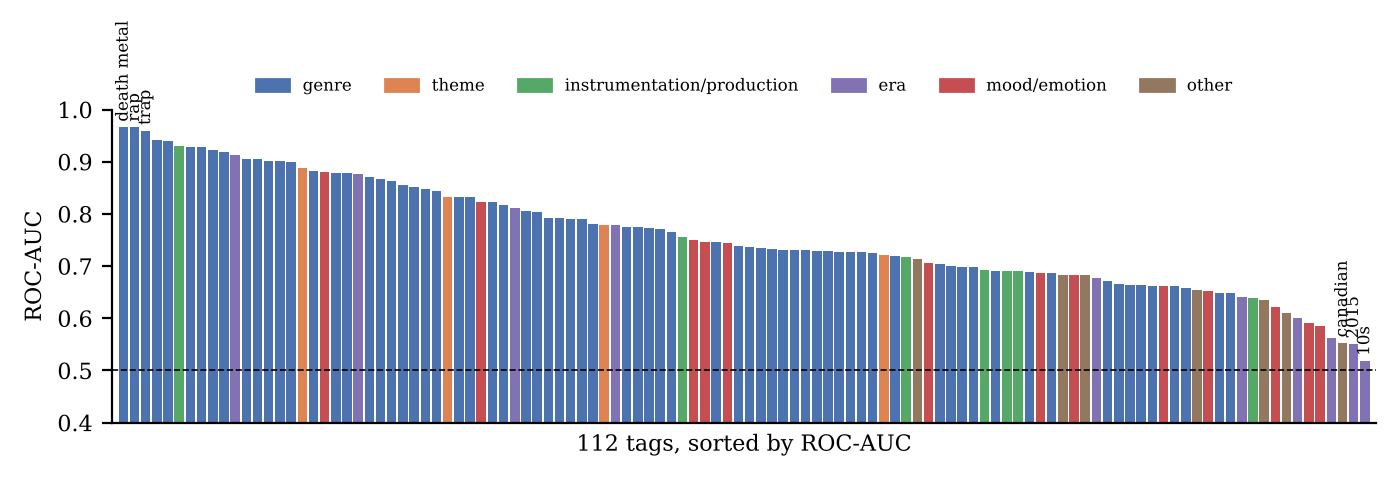
\includegraphics[width=\columnwidth]{figs/per_tag_auc.png}
\caption{Per-tag ROC-AUC of TF-IDF + LR on validation, sorted and colored by tag category.}
\label{fig:pertag}
\end{figure}

\begin{table}[t]
\centering\small
\begin{tabular}{@{}lcccc@{}}
\toprule
Category & Tags & Ma-F1 & MAP & AUC \\
\midrule
Genre & 71 & .217 & .162 & .790 \\
Theme & 4 & .060 & .103 & .806 \\
Instrumentation/prod. & 7 & .121 & .076 & .731 \\
Era & 10 & .113 & .072 & .693 \\
Mood/emotion & 13 & .022 & .021 & .703 \\
\textbf{Mood + theme (H1)} & 17 & .031 & .041 & .727 \\
\bottomrule
\end{tabular}
\caption{TF-IDF + LR by tag category (validation).}
\label{tab:categories}
\end{table}

\textbf{H1 is not supported so far.} On the planned metrics the mood + theme group scores below instrumentation/production (macro-F1 .031 vs.\ .121; MAP .041 vs.\ .076), and level on AUC (.727 vs.\ .731; \tabref{tab:categories}). Genre is predicted best: the top tags are \emph{rap} (AUC .97), \emph{hip hop}, \emph{death metal} and \emph{trap}, genres with distinctive vocabulary (\figref{fig:pertag}). The worst are mood tags (\emph{atmospheric}, \emph{chill}, \emph{dreamy}, \emph{happy}) and recent-year tags. Part of the gap is prevalence: mood tags have 24--114 validation positives against 2,455 for \emph{pop}, and MAP and F1 fall with prevalence even when ranking quality does not, whereas AUC does not. We therefore add per-category AUC as a \emph{secondary} comparison, noting that this was decided after seeing the baseline.

\textbf{Informative terms and data size.} The highest-weighted terms for \emph{christmas} are \tbd{terms}, for \emph{rap} \tbd{terms}, and for \emph{sad} \tbd{terms}, which suggests \tbd{interpretation}. Learning curves (\figref{fig:lc}) show \tbd{trend}: AUC rises from \tbd{x} with 10\% of the training artists to \tbd{y} with all of them.

\begin{figure}[t]
\centering
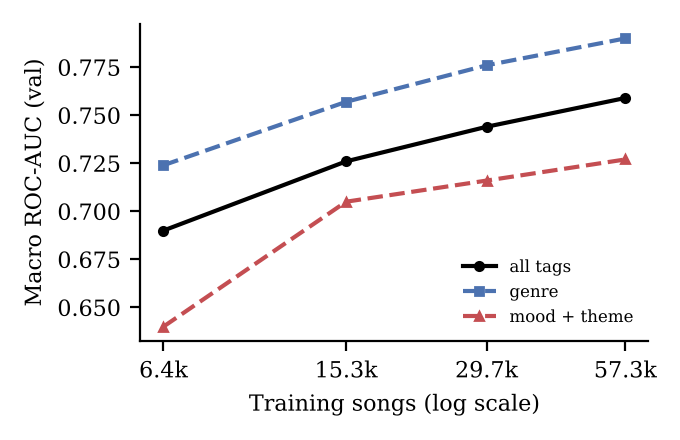
\includegraphics[width=0.85\columnwidth]{figs/learning_curve.png}
\caption{Validation macro ROC-AUC of TF-IDF + LR against training-set size (artists subsampled).}
\label{fig:lc}
\end{figure}

\textbf{Lessons learned.} Naive Bayes is weak (AUC .60) and per-tag F1 tuning drives its thresholds so low that most songs are labelled positive (Hamming loss .45), so tuned F1 is unreliable for weak models. Obtaining the dataset took longer than planned, and our Music4All-EN copy has no audio, which puts the audio baseline at risk.

%=====================================================================
\section{Individual Status Reports}\label{sec:status}

\begin{table}[t]
\centering\small
\setlength{\tabcolsep}{4pt}
\begin{tabular}{@{}llccccc@{}}
\toprule
Member & Objective & PI1 & PI2 & PI3 & PI4 & PI5 \\
 & & B & B & E & E & A \\
\midrule
Soorya & 1 Dataset & \done & \done & \done & \done & \done \\
       & 2 Baselines + harness & \done & \done & \done & \done & \done \\
       & 3 Per-tag analysis & \done & \done & \done & \done & \prog \\
\midrule
Mansoor & 1 Embeddings & \tbd{?} & \tbd{?} & \tbd{?} & \tbd{?} & \tbd{?} \\
        & 2 Classifier chains & \tbd{?} & \tbd{?} & \tbd{?} & \tbd{?} & \tbd{?} \\
        & 3 Tuning & \tbd{?} & \tbd{?} & \tbd{?} & \tbd{?} & \tbd{?} \\
\midrule
Harish & 1 Stylistic features & \tbd{?} & \tbd{?} & \tbd{?} & \tbd{?} & \tbd{?} \\
       & 2 Error analysis & \tbd{?} & \tbd{?} & \tbd{?} & \tbd{?} & \tbd{?} \\
       & 3 Audio baseline & \tbd{?} & \tbd{?} & \tbd{?} & \tbd{?} & \tbd{?} \\
\bottomrule
\end{tabular}
\caption{Performance indicators (B = basic, E = expected, A = advanced): \done\ done, \prog\ in progress, \nost\ not started. Full PI definitions are in the repository README.}
\label{tab:pis}
\end{table}

\textbf{Soorya Vasudevan} (data, baselines, evaluation). All basic and expected PIs are complete (\tabref{tab:pis}). \emph{Objective 1:} Music4All-EN is loaded and joined on song ID; filtering statistics, tag normalization, frequency and co-occurrence plots, artist-disjoint stratified splits (with a song-level split kept for the leakage check) and the documented category mapping are in the repository. \emph{Objective 2:} TF-IDF features, the popularity and random baselines, three classifiers with timing, and the retrieval metrics are implemented; the shared harness (score matrix in, metrics table out) is used by all members. \emph{Objective 3:} per-tag results sorted by AUC (\figref{fig:pertag}), informative terms, the category comparison (\tabref{tab:categories}) and learning curves (\figref{fig:lc}) are done. PI5 is in progress: bootstrap CIs are computed, and per-tag significance tests with Benjamini--Hochberg correction remain. \emph{Next:} the leakage check (artist-disjoint vs.\ song-level split) and paired bootstrap tests for RQ2 and RQ3.

\textbf{Mansoor Ali} (embeddings, classifier chains, tuning). \tbd{Mansoor: 3--4 sentences on progress for each objective, results so far, and next steps.}

\textbf{Harish Pugazhenthi Sasikala} (stylistic features, error analysis, audio baseline). \tbd{Harish: 3--4 sentences on progress for each objective, results so far, and next steps, including whether the audio clips for the 10k-song subset have been obtained.}

%=====================================================================
\section{Revised Plan and Final Goals}\label{sec:plan}

Our original timeline slipped by about a week because of dataset access; the remaining schedule is: Nov.~13--20 embeddings, classifier chains and stylistic features; Nov.~21--27 tuning, error analysis and a single test-set evaluation of the frozen models; Nov.~28--Dec.~4 final paper. Goals for the final report:

\textbf{Basic:} the frozen dataset, shared harness and TF-IDF baselines, plus a sentence-embedding model, all evaluated once on the test split, with per-category results answering RQ1 and RQ2.

\textbf{Expected:} classifier chains vs.\ binary relevance (RQ3), tuned thresholds for all models, stylistic features, error analysis of mood tags, bootstrap CIs with paired tests per research question, the leakage check, and an MFCC audio baseline on a 10k-song subset if clips are available by Nov.~13.

\textbf{Advanced:} a fine-tuned transformer, late fusion of TF-IDF and embedding models, a pretrained audio embedding with audio--lyrics fusion, and per-tag significance tests with Benjamini--Hochberg correction.

\bibliography{refs}

\end{document}
